\documentclass[11pt]{article}
\usepackage{amsmath}
\usepackage{physics}
\usepackage{amssymb}
\usepackage{graphicx}
\usepackage{hyperref}
\usepackage{amsfonts}
\usepackage{cancel}
\usepackage{xcolor}
\hypersetup{
	colorlinks,
	linkcolor={black!50!black},
	citecolor={blue!50!black},
	urlcolor={blue!80!black}
}
\newcommand{\f}[2]{\frac{#1}{#2}}
\usepackage{newpxtext,newpxmath}
\usepackage[left=1in,right=1in,top=1.25in,bottom=1.25in]{geometry}
\usepackage{framed}
\usepackage{enumerate}

\usepackage{caption}
\usepackage{subcaption}

%\newcommand{\fig}[1]{figure #1}
%\newcommand{\explain}{appendix?}
%\newcommand{\rat}{\mathbb{Q}}
%
%\newcommand{\mathbb{R}}{\mathbb{R}}
%\newcommand{\nat}{\mathbb{N}}
%\newcommand{\inte}{\mathbb{Z}}
%\newcommand{\M}{{\cal{M}}}
%\newcommand{\sss}{{\cal{S}}}
%\newcommand{\rrr}{{\cal{R}}}
%\newcommand{\uu}{2pt}
%\newcommand{\vv}{\vec{v}}
%\newcommand{\comp}{\mathbb{C}}
%\newcommand{\field}{\mathbb{F}}
%\newcommand{\f}[1]{ \hspace{.1in} (#1) }
%\newcommand{\set}[2]{\mbox{$\left\{ \left. #1 \hspace{3pt}
%\right| #2 \hspace{3pt} \right\}$}}
%\newcommand{\integral}[2]{\int_{#1}^{#2}}
%\newcommand{\ba}{\hookrightarrow}
%\newcommand{\ep}{\varepsilon}
%\newcommand{\limit}{\operatornamewithlimits{limit}}
%\newcommand{\ddd}{.1in}
%\newcommand{\ccc}{2in}
%\newcommand{\aaa}{1.5in}
%\newcommand{\B}{{\cal B}}
%\newcommand{\C}{{\cal C}}
%\newcommand{\D}{{\cal D}}
%\newcommand{\FF}{{\cal F}}
\usepackage{amssymb}% http://ctan.org/pkg/amssymb
\usepackage{pifont}% http://ctan.org/pkg/pifont
\newcommand{\cmark}{\ding{51}}%
\newcommand{\xmark}{\ding{55}}%
\newcommand{\p}{\partial}%
%\usepackage{MnSymbol,wasysym}



\usepackage{listings}
\captionsetup[lstlisting]{margin=0cm,format=hang,font=small,format=plain,labelfont={bf,up},textfont={it}}
\renewcommand*{\lstlistingname}{Code \textcolor{violet}{\textsl{Mathematica}}}
\definecolor{gris245}{RGB}{245,245,245}
\definecolor{olive}{RGB}{50,140,50}
\definecolor{brun}{RGB}{175,100,80}
\lstset{
	tabsize=4,
	frame=single,
	language=mathematica,
	basicstyle=\scriptsize\ttfamily,
	keywordstyle=\color{black},
	backgroundcolor=\color{gris245},
	commentstyle=\color{gray},
	showstringspaces=false,
	emph={
		r1,
		r2,
		epsilon,epsilon_,
		Newton,Newton_
	},emphstyle={\color{olive}},
	emph={[2]
		L,
		CouleurCourbe,
		PotentielEffectif,
		IdCourbe,
		Courbe
	},emphstyle={[2]\color{blue}},
	emph={[3]r,r_,n,n_},emphstyle={[3]\color{magenta}}
}






\begin{document}
\begin{center}
{\large \bf PH312: Physics of Fluids (Prof. McCoy) -- Reflection}\\
{ Huan Q. Bui}\\
April 2, 2021
\end{center}



\noindent \textbf{1.}


\begin{enumerate}[(a)]
	\item The solution to the PDE
	\begin{equation*}
	\p_t u = \nu \p^2_y u 
	\end{equation*}
	with initial condition
	\begin{equation*}
	u(y,0) = \begin{cases}
	+U,\quad y>0 \\
	-U,\quad  y < 0
	\end{cases}
	\end{equation*}
	is given by 
	\begin{equation*}
	u(\eta) = U \erf(\eta), \quad\quad \eta = y/\sqrt{4\nu t}.
	\end{equation*}
	Let $U = 1, \nu = 1$, we find the following space-time plots of the solution:
	\begin{figure}[!htb]
		\centering
		\begin{subfigure}{0.49\textwidth}
			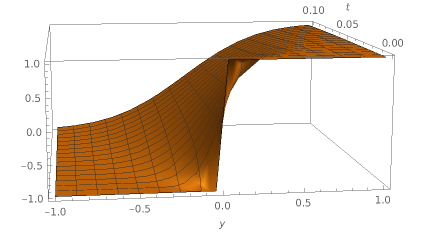
\includegraphics[scale=0.75]{1a_1}
		\end{subfigure}
		\begin{subfigure}{0.49\textwidth}
			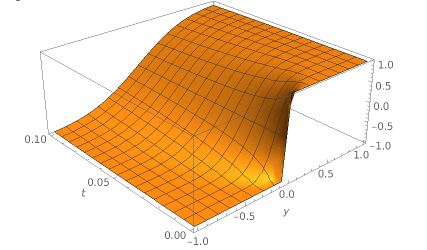
\includegraphics[scale=0.75]{1a_2}
		\end{subfigure}
	\end{figure}
	This makes sense: At $t=0$ there is a discontinuity due to the initial condition. But the solution (flow field) becomes smoother as $t$ increases. \\
	
	Mathematica code: 
	\begin{lstlisting}
	eta[y\_,t\_] = := y/Sqrt[4t]; 
	Plot3D[Erf[eta[y,t]], {y,-1,1},{t,0,1}, AxesLabel -> Automatic]
	\end{lstlisting}

	
	
	
	\item To see how $u(\eta)$ is obtained, we use the heat kernel $G$.  For each $y,t$, we set $\alpha(y') = (y-y')/\sqrt{4\nu t}$. This means that 
	\begin{equation*}
	\int_0^\infty\,dy'\dots \to -\int_{y/\sqrt{4\nu t}}^{-\infty} d\alpha \dots = +\int^{y/\sqrt{4\nu t}}_{-\infty} d\alpha \dots
	\end{equation*}
	since $y'$ carries a minus sign in $\alpha$. 
	\begin{align*}
	u(y,t) 
	&= G\ast u(y,0) \\
	&= \f{1}{\sqrt{4\nu t}}\cdot \f{1}{\sqrt{\pi}} \int^\infty_{-\infty} \exp(-\f{(y-y')^2}{4\nu t}) \cdot u(y',0)\,dy' \\
	&= \f{U}{\sqrt{4\nu t}}\cdot \f{1}{\sqrt{\pi}}\left[   
	\int_0^\infty \exp(-\f{(y-y')^2}{4\nu t}) \,dy' - \int_{-\infty}^0 \exp(-\f{(y-y')^2}{4\nu t}) \,dy'
	\right]\\
	&= \f{U}{\sqrt{\pi}}\left[ \int_{-\infty}^{y/\sqrt{4\pi t}} \exp(-\alpha^2) \,d\alpha -  
	\int_{y/\sqrt{4\pi t}}^\infty \exp(-\alpha^2) \,d\alpha
	\right]\\
	&= \f{U}{\sqrt{\pi}}\left[2\int_0^{y/\sqrt{4\nu t}} \exp(-\alpha^2)\,d\alpha \right] \equiv \f{2U}{\sqrt{\pi}}\erf\left( \f{y}{\sqrt{4\nu t}}\right),
	\end{align*}
	where we have used the symmetry of the Gaussian to cancel the integrals $-\int^\infty_0$ and $\int^0_{-\infty}$ and keep 2 terms of $\int_0^{y/\sqrt{4\nu t}}$ and the definition of the error function. 
	
	
	\item We have $\omega = \nabla \times u$. Since the curl can go through derivatives, the PDE $\p_t u = \nu \p_y^2 u$ can be transformed to $\p_t \nabla \times u = \nu \p_y^2 \nabla \times u$, which gives $\p_t \omega = \nu \p_y^2 \omega$. By the geometry of the problem, $\omega$ can be treated as a scalar field, which is the only nonzero component of the vorticity (more formally denoted by $\vec{\omega}$). With the expression for $u(\eta)$, we write
	\begin{equation*}
	\omega(y,t) = -\p_y u(y,t) = -\f{\p}{\p y}  \f{U}{\sqrt{\pi}}\left[ 2\int_0^{y/\sqrt{4\nu t}} \exp(-\alpha^2)\,d\alpha \right].
	\end{equation*}
	By Leibniz's rule for integrals we find 
	\begin{equation*}
	\omega(y,t) = \f{-2U}{\sqrt{\pi}} \exp\left(- \f{y^2}{{4\nu t}}  \right) \f{d}{dy} \f{y}{\sqrt{4\nu t}}  - 0 + \cancel{\int^{y/\sqrt{4\nu t}}_0 \f{\p}{\p y} \exp(-\alpha^2)\,d\alpha}.
	\end{equation*}
	So, 
	\begin{equation*}
	\omega(y,t) = \f{-U}{\sqrt{\pi \nu t}}\exp\left(
	- \f{y^2}{{4\nu t}}\right).
	\end{equation*}
	This is a negative Gaussian whose width is proportional to $\sqrt{t}$ and for any  $t>0$ decreases as $\abs{y}$ increases. At small $t$, the vorticity $\omega$ is highly concentrated near the origin. As $t$ increases, $\omega$ away \textit{diffuses} towards infinity. At any $t>0$, the total vorticity is $\int_{\mathbb{R}} \omega\,dy$. Since $\omega$ is a scaled Gaussian, $\int_{\mathbb{R}} \omega\,dy$ is a constant depending only on $U$ (since $\nu$ can be absorbed into $t$, the analogue of the standard deviation). We therefore conclude that the total amount of vorticity is constant.   
	
	
	\item Starting with $\omega = -2U \delta(y)$ at $t=0$, we find 
	\begin{align*}
	\omega(y,t) &=  -2U \cdot G\ast\delta(y) =  -2U\cdot  G(y,t) \\
	&= \f{-2U}{\sqrt{4\pi \nu t}}\exp\left( -\f{y^2}{4\nu t} \right) = \f{-U}{\sqrt{\pi \nu t}}\exp\left(
	- \f{y^2}{{4\nu t}}\right),
	\end{align*}
	since convolving $G$ with the delta function is an evaluation of $G$ at $y'=0$. 
\end{enumerate}




\noindent \textbf{2.}
\begin{enumerate}[(a)]
	\item To derive the stream function K\&C 9.64, we start by taking the curl on both sides of $\nabla p = \mu \laplacian \mathbf{u}$. This gives $0 = \laplacian \mathbf\omega$, since $\nabla p$ is conservative. Next, since the nonzero components of the flow field $\mathbf{u}$ are $u_r$ and $u_\theta$, there is only one nonzero component of $\mathbf\omega$, which is the axial $\omega_\varphi$ (right-hand rule). The spherical curl gives us $\omega_\varphi$ in terms of $u_r,u_\theta$. \\
	
	Next, since we're in axisymmetric flow, a stream function $\psi$ can be defined  such that $\mathbf{u} = -\nabla \varphi \times \nabla \psi$, which allows us to write $u_r$ and $u_\theta$ in terms of derivatives $\psi$. With this, we can write $\omega_\varphi$ in terms of derivatives of $\psi$. From $\laplacian \omega = 0$, we obtain (9.64). 
	
	\item With 
	\begin{equation*}
	\psi(r,\theta) = Ur^2 \sin^2\theta \left[ \f{1}{2} - \f{3a}{2r} + \f{a^3}{4r^3} \right],
	\end{equation*}
	we find 
	\begin{align*}
	u_r 
	&= \f{1}{r^2\sin\theta}\p_\theta \psi\\
	&= \f{1}{r^2\sin\theta} \p_\theta\left\{ Ur^2 \sin^2\theta \left[ \f{1}{2} - \f{3a}{4r} + \f{a^3}{4r^3} \right] \right\}\\
	&= \f{2Ur^2\sin\theta\cos\theta}{r^2\sin\theta}\left[ \f{1}{2} - \f{3a}{4r} + \f{a^3}{4r^3} \right] \\
	&= U\cos\theta \left[ 1 - \f{3a}{2r} + \f{a^3}{2r^3} \right]
	\end{align*}
	and
	\begin{align*}
	u_\theta 
	&= -\f{1}{r\sin\theta}\p_r \psi\\
	&= -\f{1}{r\sin\theta}\p_r \left\{ Ur^2 \sin^2\theta \left[ \f{1}{2} - \f{3a}{4r} + \f{a^3}{4r^3} \right] \right\}\\
	&= -\f{U\sin^2\theta}{r\sin\theta}\left[ r - \f{3ar}{4r} - \f{ra^3}{4r^3}  \right]\\
	&= -U\sin\theta\left[ 1 - \f{3a}{4r} - \f{a^3}{4r^3}  \right].
	\end{align*}
	
	
	\item We have $\nabla p = \mu\laplacian \mathbf{u}$, so we need to take the spherical laplacian of $\mathbf{u}$. While one can try to do this by hand using the formula of laplacian for a vector in the Appendix of K\&C (which can be quite tedious), we can also do this in Mathematica:

	\begin{lstlisting}
	Ur[r_,\[Theta]_,\[Phi]_]:=U*Cos[\[Theta]]*(1-3a/(2r)+a^3/(2r^3) );
	U\[Theta][r_,\[Theta]_,\[Phi]_]:= -U*Sin[\[Theta]]*(1-3a/(4r)-a^3/(4r^3));
	U\[Phi][r_,\[Theta]_,\[Phi]_] :=0;
	
	Laplacian[{Ur[r,\[Theta],\[Phi]], U\[Theta][r,\[Theta]
	,\[Phi]], U\[Phi][r,\[Theta],\[Phi]]}, {r, \[Theta], \[Phi] },
	 "Spherical"] //Expand//MatrixForm 
	\end{lstlisting}	
	to find
	\begin{equation*}
	\nabla p = \laplacian \mathbf{u} = 
	\begin{pmatrix}
	\frac{3aU\cos\theta}{r^3}&
	\frac{3aU\sin\theta}{2r^3}&
	0
	\end{pmatrix}^\top.
	\end{equation*} 
	Taking the spherical gradient of $p$, we find the following equations:
	\begin{equation*}
	\p_r p = \frac{3aU\cos\theta}{r^3}\quad \text{and} \quad
	\f{1}{r}\p_\theta p = \frac{3aU\sin\theta}{2r^3}.
	\end{equation*}
	Using the method of inspection \footnote{more commonly known as ``equation staring''} and setting the integration constant to be $p_\infty$, we get the following expression for $p$:
	\begin{equation*}
	p = -\mu U \cos\theta \f{3a}{2r^2}.
	\end{equation*}
	We remark that this expression is analogous to the \textcolor{purple}{electric potential due to a small dipole} in electrostatics: $V = kp\cos\theta/r^2$ where $\vec{p} = q\vec{d}$ is the electric dipole moment.
	
	
	\item Now we calculate the stress components:
	\begin{equation*}
	\sigma_{rr}  = 2\mu \p_r u_r = 2\mu U\cos\theta \left[\f{3a}{2r^2} - \f{3a^3}{2r^4}\right]
	\end{equation*}
	and 
	\begin{equation*}
	\sigma_{r\theta} = \mu \left[r\p_r(u_\theta/r) + (1/r)\p_\theta u_r\right] = -\f{3\mu Ua^3}{2r^4}\sin\theta.
	\end{equation*}
	With these, we can compute the component of the drag force per unit area in the direction of the uniform stream:
	\begin{align*}
	[-p\cos\theta + \sigma_{rr}\cos\theta - \sigma_{r\theta}\sin\theta]_{r=a} &=  \f{3a\mu U \cos^2\theta}{2a^2} + \cancel{2\mu U\cos^2\theta \left[\f{3a}{2a^2} - \f{3a^3}{2a^4}\right]} + \f{3\mu Ua^3\sin^2\theta}{2a^4}\\
	&=  \cos^2\theta \f{3 \mu U}{2a} + \sin^2\theta\f{3\mu U}{2a}\\
	&= \f{3\mu U }{2a}.
	\end{align*}
	Integrating this (a constant) over the surface of the sphere is just multiply it by the surface area $4\pi a^2$ of the sphere, so the total force is
	\begin{equation*}
	F = \f{3\mu U }{2a}\times 4\pi a^2 = 6\pi \mu a U.
	\end{equation*}
	We have just derived Stokes' law of resistance!
\end{enumerate}




\end{document}




